\documentclass[a4paper,10pt]{article}

\usepackage[margin=16mm]{geometry}
\usepackage{hyperref}
\usepackage{indentfirst}
\usepackage{tikz}

\title{Stealth Address}
\author{Sammy}
\date{2017-09-22}

\hypersetup{
    colorlinks=true,
    linkcolor=blue,
    filecolor=magenta,      
    urlcolor=cyan,
}
\urlstyle{same}
\usetikzlibrary{arrows,decorations.pathmorphing,positioning,fit,petri}

\begin{document}
\maketitle

\section{Definitions}
Stealth addressing is a technique whereby a \textbf{sender} can take a \textbf{recipient}'s public address and transform it to a one-time address such that:
	\begin{itemize}
		\item For anyone other than the recipient, the address is
			\begin{itemize}
				\item \textbf{publicly unlinkable} to the original public address;
				\item \textbf{publicly unlinkable} to \textbf{any} other one-time address;
			\end{itemize}
		\item The recipient can
			\begin{itemize}
				\item link all their payments together 
				\item derive the secret key associated with the one-time address
			\end{itemize}
	\end{itemize}
Using stealth addressing, a recipient can publish one address and receive unlimited publicly unlinkable payments.
\section{Requisites -- ECDH}
\href{https://en.wikipedia.org/wiki/Elliptic_curve_Diffie%E2%80%93Hellman}{Elliptic Curve Diffie-Hellman} is a variant of the original \href{https://en.wikipedia.org/wiki/Diffie%E2%80%93Hellman_key_exchange}{Diffie-Hellman} key agreement protocol extended for use with \href{https://en.wikipedia.org/wiki/Elliptic_curve_cryptography}{ECC}. In simple terms, two parties can independently generate a shared secret over an unsecured connection (implying that no observer can discover the secret by simply watching their communication). \par
	Suppose the two parties to share secret keys are Alice and Bob, and their \((sk,pk)\) pair are \( (a,A=a\cdot G)\) and \( (b,B=b\cdot G)\) respectively, where \(G\) is a base point of the EC employed.\par
\begin{figure}[!htbp]
	\centering
	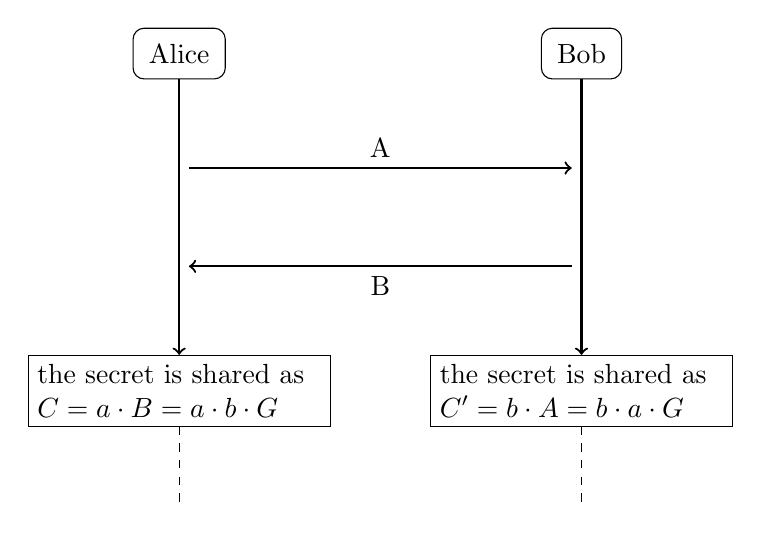
\begin{tikzpicture}[auto,
		place/.style={rectangle,draw},
		marrow/.style={->,thick}]
		\node [place,rounded corners,inner sep=2mm] (alice) {Alice};
		\node [place,rounded corners,inner sep=2mm] (bob) [right=4cm of alice]  {Bob};

		\node (A-send) [below=of alice] {};
		\node (A-recv) [below=of bob] {};

		\node (B-send) [below=of A-recv] {};
		\node (B-recv) [below=of A-send] {};

		\node [place] (C-calc) [below=of B-recv,text width=36mm] {
			the secret is shared as
			\( C=a\cdot B=a\cdot b\cdot G \) 
		};
		\node [place] (C-pi-calc) [below=of B-send,text width=36mm] {
			the secret is shared as
			\( C'=b\cdot A=b\cdot a\cdot G \) 
		};

		\node (alice-end) [below=of C-calc] {};
		\node (bob-end) [below=of C-pi-calc] {};

		% horizontal arrows
		\draw [marrow] (A-send) to node [align=center] {A} (A-recv);
		\draw [marrow] (B-send) to node [align=center] {B} (B-recv);
	
		% vertical arrows
		\draw [marrow] (alice) to (C-calc);
		\draw [-,dashed] (C-calc) to (alice-end);

		\draw [marrow] (bob) to (C-pi-calc);
		\draw [-,dashed] (C-pi-calc) to (bob-end);
	\end{tikzpicture}
	\caption{Workflow of ECDH}
\end{figure}
And the final shared secret key is \(C=C'\).

\end{document}
